\documentclass{beamer}
\usepackage{../../shared/styles/custom}
\usepackage{../../shared/styles/conventions}

%\beamerdefaultoverlayspecification{<+->}
% \newcommand{\data}{\mathcal{D}}
% \newcommand\Item[1][]{%
% 	\ifx\relax#1\relax  \item \else \item[#1] \fi
% 	\abovedisplayskip=0pt\abovedisplayshortskip=0pt~\vspace*{-\baselineskip}}

\title{Logistic Regression}
\date{\today}
\author{Nipun Batra}
\institute{IIT Gandhinagar}
\begin{document}
\maketitle

\begin{frame}Aim: Probability(Tomatoes $|$ Radius) ? or
	\pause \framebox{More generally, P($y = 1 | \mX = \vx$)?}
	
\end{frame}

\begin{frame}Generally,
\begin{equation*}
P(y = 1 | \vx) = \mX\vtheta
\end{equation*}
\end{frame}
\begin{frame}$\sigma(z) \rightarrow 1$\\
\pause $z \rightarrow -\infty$\\
 \pause $\sigma(z) \rightarrow 0$\\
 \pause $z = 0$\\
 \pause $\sigma(z) = 0.5$

\end{frame}

\begin{frame}\begin{equation*}
P(y = 0 | X) = 1 - P(y = 1 | X) = 1 - \frac{1}{1 + e^{-\mX\vtheta}} = \frac{e^{-\mX\vtheta}}{1 + e^{-\mX\vtheta}} 
\end{equation*}

\pause \begin{equation*}
\therefore \frac{P(y = 1|X)}{1 - P(y = 1|X)} = e^{\mX\vtheta}
\implies \mX\vtheta = \log\frac{P(y = 1|X)}{1 - P(y = 1 | X)}
\end{equation*}
\end{frame}
\begin{frame}\textbf{Why?} Squared loss + sigmoid creates non-convex surface:
\begin{itemize}
\item Sigmoid $\sigma(z) = \frac{1}{1+e^{-z}}$ is non-linear
\item Composition $(\sigma(\mX\vtheta) - y)^2$ has multiple local minima
\pause
\item No guarantee gradient descent finds global optimum
\item \textcolor{red}{This is why we need cross-entropy loss instead!}
\end{itemize}
\end{frame}

\section{Deriving Cost Function via Maximum Likelihood Estimation}

\begin{frame}This cost function is called cross-entropy.

\pause Why?
\end{frame}

\begin{frame}What is the interpretation of the cost function?

\pause Let us try to write the cost function for a single example:

\pause $$J(\theta) = -y_i\log{\hat{y}_i} - (1-y_i)\log({1-\hat{y}_i})$$

\pause First, assume $y_i$ is 0, then if $\hat{y}_i$ is 0, the loss is 0; but, if $\hat{y}_i$ is 1, the loss tends towards infinity!

	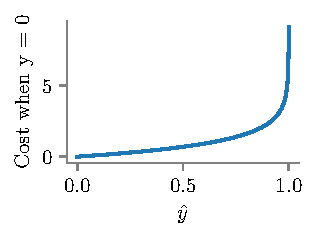
\includegraphics[scale=0.7]{../assets/logistic-regression/figures/logistic-cross-cost-0}

\end{frame}

\begin{frame}What is the interpretation of the cost function?

 $$J(\theta) = -y_i\log{\hat{y}_i} - (1-y_i)\log({1-\hat{y}_i})$$

\pause Now, assume $y_i$ is 1, then if $\hat{y}_i$ is 0, the loss is huge; but, if $\hat{y}_i$ is 1, the loss is zero!

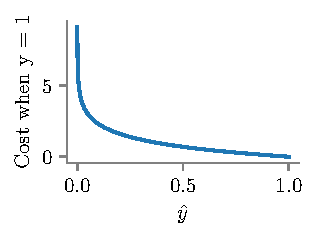
\includegraphics[scale=0.7]{../assets/logistic-regression/figures/logistic-cross-cost-1}

\end{frame}

\begin{frame}Bias! 
\end{frame}

\begin{frame}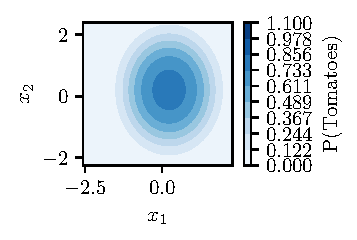
\includegraphics{../assets/logistic-regression/figures/logisitic-circular-probability.pdf}

\end{frame}

\begin{frame}How would you learn a classifier? Or, how would you expect the classifier to learn decision boundaries?
\end{frame}

\begin{frame}\begin{enumerate}
\item Use one-vs.-all on \underline{Binary} Logistic Regression
\item Use one-vs.-one on \underline{Binary} Logistic Regression
\item Extend \underline{Binary} Logistic Regression to \underline{Multi-Class} Logistic Regression
\end{enumerate}
\end{frame}

\begin{frame}\begin{enumerate}
	\item Learn P(setosa (class 1)) = $\mathcal{F}({\mX\vtheta_1})$
	\item P(versicolor (class 2)) = $\mathcal{F}({\mX\vtheta_2})$
	\item P(virginica (class 3)) = $\mathcal{F}({\mX\vtheta_3})$
	\item Goal: Learn $\theta_i \forall i \in \{1, 2, 3\}$
	\item Question: What could be an $\mathcal{F}?$

\end{enumerate}

\end{frame}

\begin{frame}\begin{enumerate}
	\item Question: What could be an $\mathcal{F}?$
	\item Property: $\sum_{i=1}^{3}\mathcal{F}{({\mX\vtheta_i})} = 1$
	\item Also $\mathcal{F}(z)\in [0, 1]$
	\item Also, $\mathcal{F}(z)$ has squashing proprties: $R \mapsto [0, 1]$
\end{enumerate}

\end{frame}
\begin{frame}Let us calculate $-\sum_{k=1}^{3}y_i^k \log{\hat{y}_i^k} $

\pause  = $-(0\times \log(0.1) + 1\times \log(0.8) + 0\times \log(0.1))$

\pause Tends to zero

\end{frame}

\begin{frame}Let us calculate $-\sum_{k=1}^{3}y_i^k \log{\hat{y}_i^k} $

\pause  = $-(0\times \log(0.1) + 1\times \log(0.4) + 0\times \log(0.1))$

\pause High number! Huge penalty for misclassification!

\end{frame}

\begin{frame}More generally, 
\pause \begin{equation*}
J(\theta) = -\bigg\{\sum_{i=1}^{N}y_{i}\log(\hat{y}_i) + (1 - y_{i})\log(1 - \hat{y}_i)\bigg\}
\end{equation*}

\pause \begin{equation*}
J(\theta) = -\bigg\{\sum_{i=1}^{N}y_{i}\log(\hat{y}_i) + (1 - y_{i})\log(1 - \hat{y}_i)\bigg\}
\end{equation*}

Extend to K-class:
\begin{equation*}
J(\theta) = -\bigg\{\sum_{i=1}^{N}\sum_{k=1}^{K}y_{i}^k\log(\hat{y}_{i}^k)\bigg\}
\end{equation*}
\end{frame}
\begin{frame}\item What is the key difference between sigmoid and softmax functions?
\pause
\item Why do we use cross-entropy loss instead of squared error?
\pause
\item How does regularization help in logistic regression?
\end{enumerate}
\end{frame}

\begin{frame}{Key Takeaways}
\begin{itemize}
\item \textbf{Probabilistic Model}: Outputs probabilities via sigmoid function
\pause
\item \textbf{Linear Decision Boundary}: Creates linear separation in feature space
\pause
\item \textbf{Maximum Likelihood}: Optimized using gradient-based methods
\pause
\item \textbf{Cross-Entropy Loss}: Appropriate for classification problems
\pause
\item \textbf{No Closed Form}: Requires iterative optimization (gradient descent)
\pause
\item \textbf{Regularization}: L1/L2 help prevent overfitting
\end{itemize}
\end{frame}

\end{document}
